\documentclass{article}

% if you need to pass options to natbib, use, e.g.:
%     \PassOptionsToPackage{numbers, compress}{natbib}
% before loading neurips_2019

% ready for submission
% \usepackage{neurips_2019}

% to compile a preprint version, e.g., for submission to arXiv, add add the
% [preprint] option:
%     \usepackage[preprint]{neurips_2019}

% to compile a camera-ready version, add the [final] option, e.g.:
     \usepackage[final]{neurips_2019}

% to avoid loading the natbib package, add option nonatbib:
%     \usepackage[nonatbib]{neurips_2019}

\usepackage[utf8]{inputenc} % allow utf-8 input
\usepackage[T1]{fontenc}    % use 8-bit T1 fonts
\usepackage{hyperref}       % hyperlinks
\usepackage{url}            % simple URL typesetting
\usepackage{booktabs}       % professional-quality tables
\usepackage{amsfonts}       % blackboard math symbols
\usepackage{nicefrac}       % compact symbols for 1/2, etc.
\usepackage{microtype}      % microtypography
\usepackage{graphicx}
\usepackage{subfig}
\usepackage{algpseudocode,algorithm}
\usepackage{multicol}
\usepackage{hyperref}
\hypersetup{
    colorlinks=true,
    linkcolor=blue,
    filecolor=magenta,      
    urlcolor=cyan,
}
\usepackage{caption}
\captionsetup[table]{labelsep=space}
\captionsetup[figure]{labelsep=space}

\newcommand{\mycaption}[2]{\caption[#1]{\textbf{#1.} #2}}

\title{Implementing GAN on MNIST and SVHN}

% The \author macro works with any number of authors. There are two commands
% used to separate the names and addresses of multiple authors: \And and \AND.
%
% Using \And between authors leaves it to LaTeX to determine where to break the
% lines. Using \AND forces a line break at that point. So, if LaTeX puts 3 of 4
% authors names on the first line, and the last on the second line, try using
% \AND instead of \And before the third author name.

\author{%
  Shengjie Sun \\
  ss5593\\
  Department of Statistics\\
  Columbia University\\
  New York, NY 10027 \\
  \texttt{ss5593@columbia.edu} \\
  % examples of more authors
  \And
  Zeyu Yang \\
  zy2327 \\
  Department of Statistics\\
  Columbia University\\
  New York, NY 10027 \\
  \texttt{zy2327@columbia.edu}
}

\begin{document}

\maketitle

\begin{abstract}
  We implemented DCGAN and WGAN on both MNIST and SVHN datasets.
  We set up the convolution layers for the generator and discriminator and wrote the loss function for both models.
  We also tuned the some selected hyperparameters.
  The images generated by both models and datasets are quite satisfying especially for MNIST due to its simplicity of the dataset.
\end{abstract}

\section{Introduction}

Generative Adversarial Nets (GAN), first introduced by Ian Goodfellow in 2014[1], is a model that can be used to generate new images. 
It has been a hot topic since then.

The core idea of GAN is to create a two-player game: build a generator that creates fake images while the discriminator tells whether the image is true or fake. Through the training process, the ability of both generator and discriminator will increase simultaneously by fighting with each other.

The optimum case is that the generate can fully recover the distribution of the data and even the best discriminator cannot tell whether the image is fake or not i.e. the output of discriminator is $1/2$. 

To review our whole work, we recommend to refer to our github repository at \href{https://github.com/Shengjie-Sun/GR5242-FP-GAN}{https://github.com/Shengjie-Sun/GR5242-FP-GAN} besides the well documented Jupyter Notebook.

\section{Implementation DCGAN on MNIST}

MNIST dataset is a dataset of handwritten images, including 60,000 training images and 10,000 testing images.
All digits have been size-normalized and centered in a $28\times 28$ fixed-size image[2].

The dataset has been generally used to conduct pattern recognition. 
In this project, however, we will use the training image to train our GAN model and generate similar images.

\subsection{Architecture}

We use Deep Convoltional GAN (DCGAN)[4] as our structure.
It has plenty convolutional layers and does not have max pooling layer.
We mainly use transpose convolutional layer to perform upsampling in our model.

\subsubsection{Generator}

The input of the first dense layer is a $100\times 1$ random noise vector. 
We project it to $12,544$ neurons, apply batch normalization and activation function Leaky Relu, and reshape it to $7\times 7\times 256$.

The second Convoltional Transpose layer shrinks the size of filter and outputs $7\times 7\times 128$.

The third and fourth Convolutional layers have stride 2 and padding \textit{same}. They alter the first two dimensions of the input and make the input from $7\times 7$ to $14\times 14$ to $28\times 28$.
The filter makes the third dimension from 128 to 64 to 1.Thus the final output is a $28\times 28\times 1$ black and white image.

\subsubsection{Discriminator}

The discriminator takes in a $28\times 28\times 1$ array. After three convolutional layers and one dense layer, the output will be a scalar.
This scalar will be applied to a logistics function in future steps to be a probability that lies between 0 and 1. It is the probability of the input being a true image or a fake image.


\begin{multicols*}{2}
\textbf{Generator}
 \begin{itemize}
  \item First layer: Dense
    \begin{itemize}
      \item Input: $100 \times 1$ vector
      \item Units: $12,544$
      \item Batch normalization
      \item Activation: leaky relu
      \item Reshape $12,544$ to $7\times 7\times 256$
    \end{itemize}
  \item Second layer: Conv2DTranspose
    \begin{itemize}
      \item Input $7\times 7\times 256$
      \item Filter: 128
      \item Kernel size: 5
      \item Stride: 1
      \item Padding: same
      \item Batch normalization
      \item Activation: leaky relu
  \end{itemize} 
  \item Third layer: Conv2DTranspose
    \begin{itemize}
      \item Input $7\times 7\times 128$
      \item Filter: 64
      \item Kernel size: 5
      \item Stride: 2
      \item Padding: same
      \item Batch normalization
      \item Activation: leaky relu
    \end{itemize}   
  \item Fourth layer: Conv2DTranspose
    \begin{itemize}
      \item Input $14\times 14\times 64$
      \item Filter: 1
      \item Kernel size: 5
      \item Stride: 2
      \item Padding: same
      \item Activation: tanh
      \item Output $28\times 28\times 1$
    \end{itemize}   
\end{itemize}

\vfill\null
\columnbreak

\textbf{Discriminator}
\begin{itemize}
  \item First layer: Conv2D
    \begin{itemize}
      \item Input: $28 \times 28\times 1$ array
      \item Filter: 64
      \item Kernel size: 5
      \item Stride: 2
      \item Padding: same
      \item Activation: leaky relu
      \item Dropout: 0.3
  \end{itemize} 
  \item Third layer: Conv2D
    \begin{itemize}
      \item Filter: 128
      \item Kernel size: 5
      \item Stride: 2
      \item Padding: same
      \item Activation: leaky relu
      \item Dropout: 0.3
    \end{itemize}   
  \item Fourth layer: Conv2D
    \begin{itemize}
      \item Filter: 256
      \item Kernel size: 5
      \item Stride: 2
      \item Padding: same
      \item Activation: leaky relu
      \item Dropout: 0.3
    \end{itemize} 
  \item Fifth layer: Flatten
  \item Sixth layer: Dense with output $1\times 1$
\end{itemize}
\end{multicols*}

\subsubsection{Hyperparameters}

\begin{itemize}
  \item Epoch: 100
  \item Batch: 256
  \item Learning rate
    \begin{itemize}
      \item Generator: 1e-3
      \item Discriminator: 1e-4
    \end{itemize}
\end{itemize}

We have experimented on different bacthes and epoches and we believe a batch of 256 samples and 100 epoches already produced satisfying result. 
In fact, the quality of the image does not seem to have significant improvement after 50 epoches.

The reason why we choose the learning rate for the discriminator 10 times smaller than the learning rate for generator is because the discriminator is much easier to train compared with generator and giving a smaller learning rate and make the training process more stable.

Actually, the MNIST dataset is fairly simple and the normal parameters setting is good enough and no elaborate hyper-parameters tuning is required.

\subsection{Result}

\subsubsection{Tensorboard}

\begin{figure}[!htb]
  \centering
  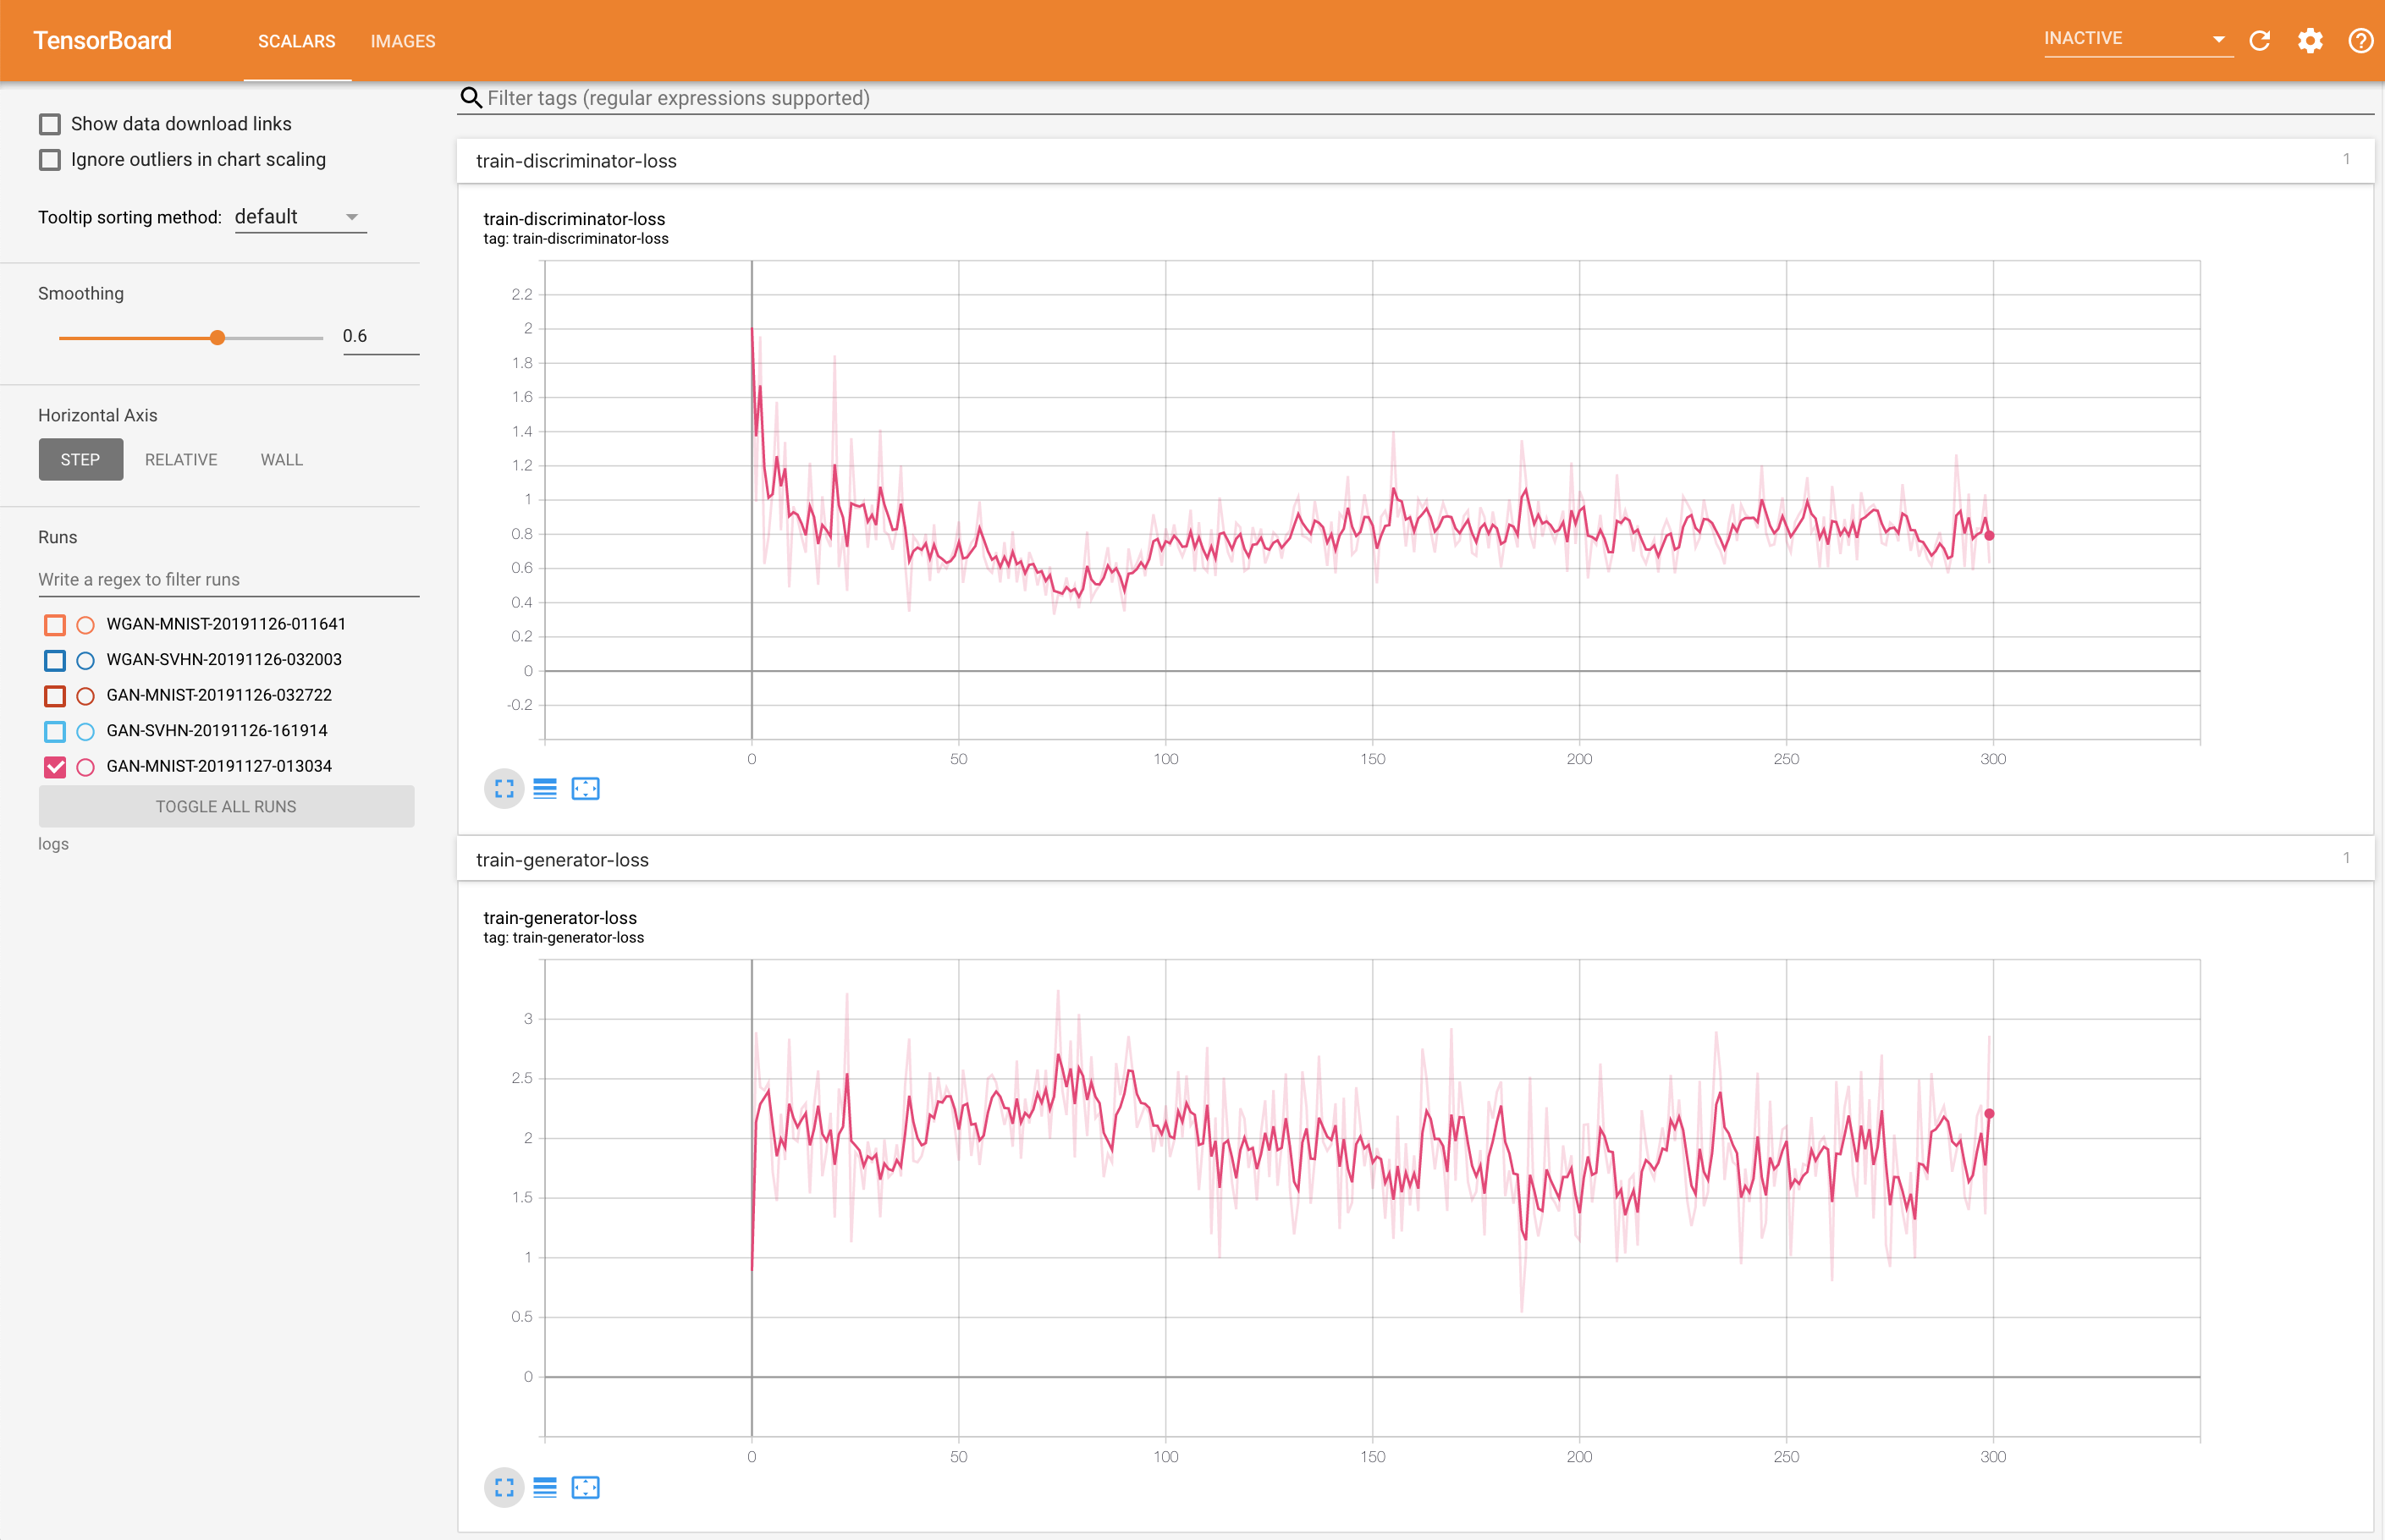
\includegraphics[width=0.8\textwidth]{imgs/tensorboard-GAN-MNIST.png}
  \mycaption{Tensorboard GAN MNSIT}{}
  \label{fig:TB_GAN_MNSIT}
\end{figure}

As we can observe from Figure \ref{fig:TB_GAN_MNSIT}, training loss of both generator and discriminator is fluctuating. 
And generally when the loss of generator decreases, the loss of discriminator increases. This is the representation of the two player game i.e. both players want to minimize their own loss.

Although the loss remains around the same level and does not continue decrease, the quality of the images are in fact improving as we can see in the following section.

\newpage
\subsubsection{Generated samples}

\begin{figure}[!htb]
  \centering
  \subfloat[MNIST data]{
  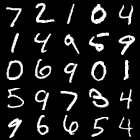
\includegraphics[width=0.2\textwidth]{imgs/mnist_data.png}}
  \subfloat[Epoch 10/100]{
  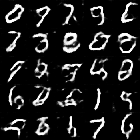
\includegraphics[width=0.2\textwidth]{imgs/I1.png}}
  \subfloat[Epoch 30/100]{
  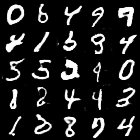
\includegraphics[width=0.2\textwidth]{imgs/I2.png}}
  \subfloat[Epoch 100/100]{
  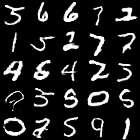
\includegraphics[width=0.2\textwidth]{imgs/I4_after-296-batches.png}}
  \mycaption{Comparison of MNIST data and generated samples from DCGAN}{}
  \label{fig_DCGAN_MNIST}
\end{figure}

From Figure \ref{fig_DCGAN_MNIST}, 
we can see the generated samples has a good approximation after 30 epoches.
The samples from the 10th are quite blury and they cannot have a good representation of number 2, 5, 8, etc.
The latter samples are clearer and the edges of the numbers are smoother.

\begin{figure}[!htb]
  \centering
  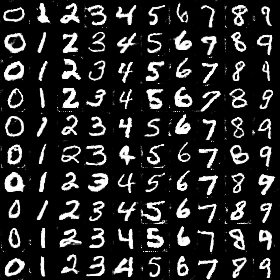
\includegraphics[width=0.5\textwidth]{imgs/MNIST_digits.png}
  \mycaption{MNSIT GAN generated digits}{}
  \label{fig_MNSIT_digits}
\end{figure}

From the generated images\ref{fig_MNSIT_digits}, we pick out some representive samples for each digit. We find out that 

a) some digits such as 5 and 8 have some redundant white marks around the edges. This is a huge difference from the original MNIST dataset whose images are clear and sharp. If discriminator could capture this difference, it might have a better judgement between true images and fake ones.

b) some digits such as 4, 1, 8 is easier to be generated while 2 and 3 is harder to be generated. This conclusion is drawn from the fact that we go through more images to find a good sample of 2 and 3. But it might be because the some digits take up more feaible space of the input noise. We cannot know for sure.

c) Digit 9 tends to transform to other digits. For example, the 1st 9 looks a little like 7 and the 4th 9 looks a little like 8.

Although not all samples are of high quality, there are a proportion of the images that have the quality of the samples presented in paper[1] 2(a).

\newpage
\section{Implementation DCGAN on SVHN}

SVHN dataset is a dataset similar to MNIST, but more challenging, containing real-world digit images that obtained from house numbers in Google Street View images. The images have been cropped into $32\times 32$ fixed-size array with three channels[3].

The challenge of implementing GANs on SVHN images is that generally the quality/resolution of the images are low. Compared to MNIST, there are more colors such as red and blue instead of black and white. The fonts/patterns are varied and thus far more harder for a generators to find/learn the ground-truth distribution of the data.

\subsection{Architecture}

\subsubsection{Generator}

The generator is slightly modifed from the generator for MNIST. 
The output of the first dense layer is changed to $8\times 8\times 256$ 
and the filter of the fourth layer (Conv2DTranspose) has changed from 1 to 3
so that the output of the whole generator would be a $32\times 32\times 3$ image.

\subsubsection{Discriminator}

Discriminator is exactly the same as the previous one except the input is $32\times 32\times 3$ instead of $28\times 28\times 1$.

\subsubsection{Hyperparameters}

\begin{itemize}
  \item Epoch: 200
  \item Batch: 256
  \item Learning rate
    \begin{itemize}
      \item Generator: 1e-3
      \item Discriminator: 1e-4
    \end{itemize}
\end{itemize}

Since the SVHN dataset is more complicated, we train the model with 200 epoches.

\subsection{Result}

\subsubsection{Tensorboard}

\begin{figure}[!htb]
  \centering
  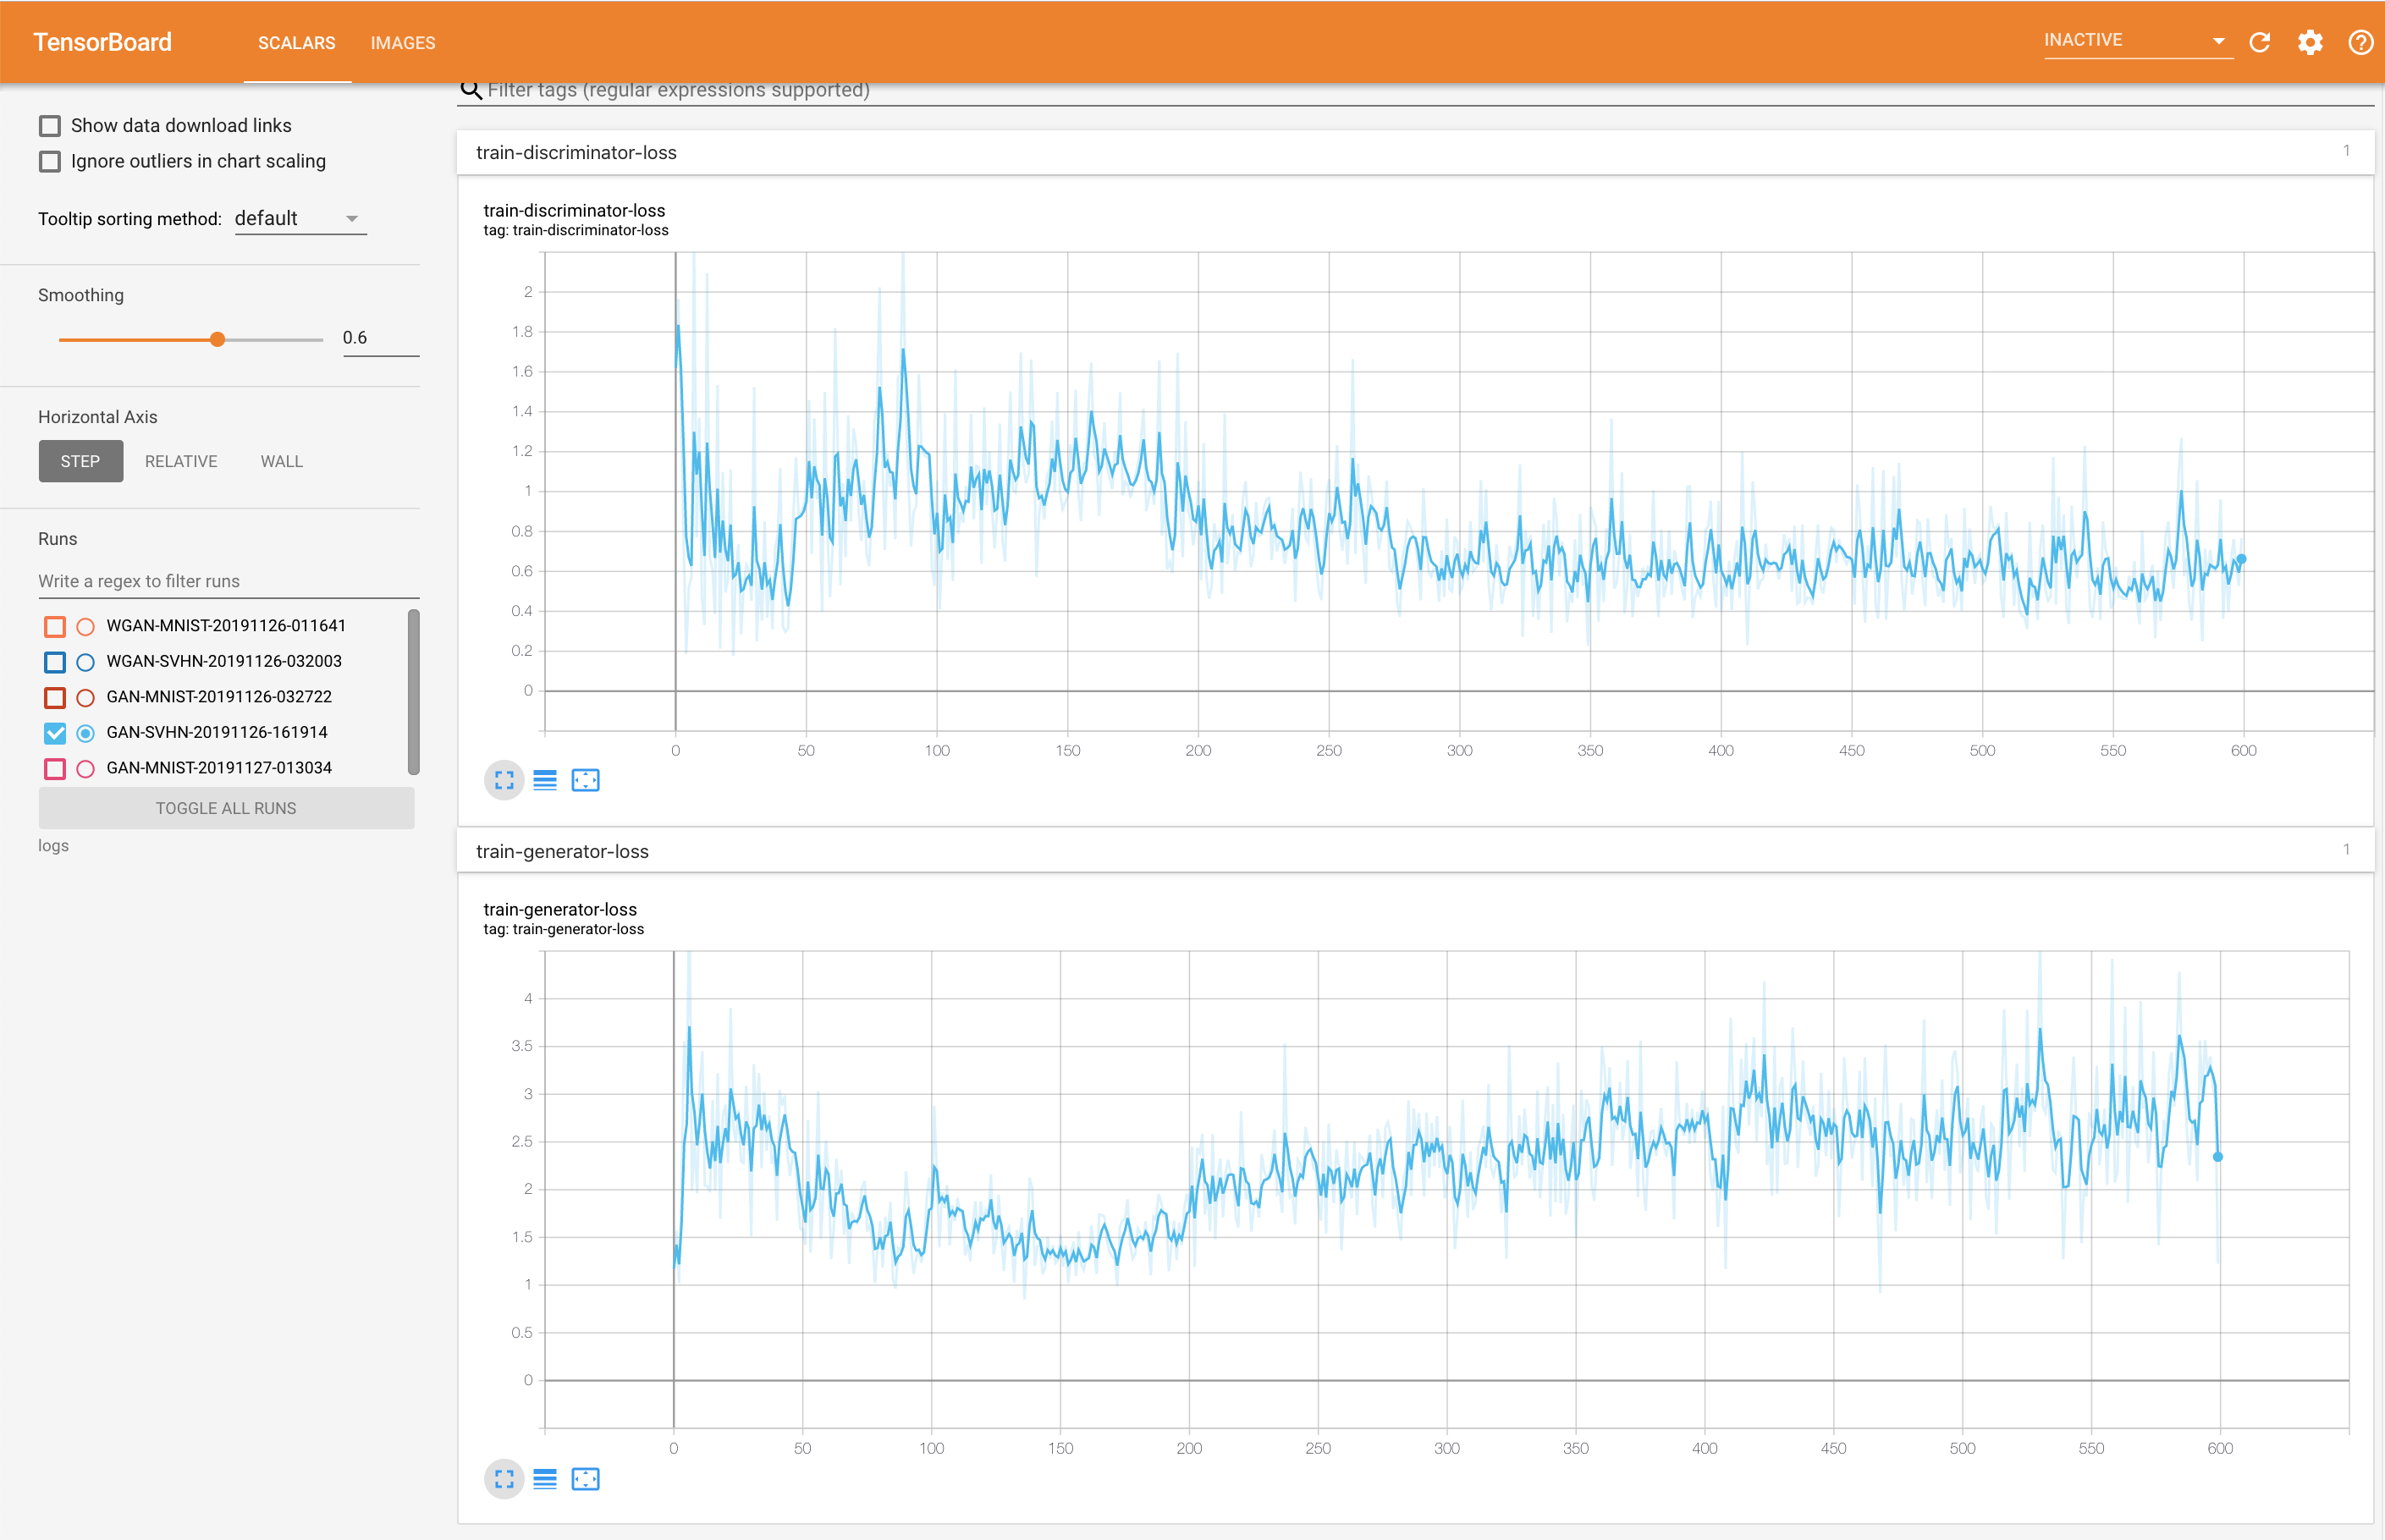
\includegraphics[width=0.8\textwidth]{imgs/tensorboard-GAN-SVHN.png}
  \mycaption{Tensorboard GAN SVHN}{}
  \label{fig_TB_GAN_SVHN}
\end{figure}

The training loss is fluctuating as well. We can see from Figure \ref{fig_TB_GAN_SVHN} that the training loss of the discriminator keeps increasing after 150 steps (50 epoches). This implies that the generator can generate the samples so well that the discriminator can hardly distinguish the true and fake image.

\subsubsection{Generated samples}

\begin{figure}[!htb]
  \centering
  \subfloat[SVHN data]{
  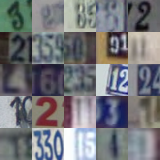
\includegraphics[width=0.2\textwidth]{imgs/svhn_data.png}}
  \subfloat[Epoch 30/200]{
  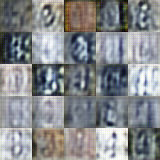
\includegraphics[width=0.2\textwidth]{imgs/s1_after-103-batches.png}}
  \subfloat[Epoch 150/200]{
  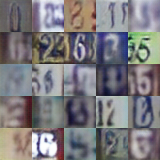
\includegraphics[width=0.2\textwidth]{imgs/s2_after-514-batches.png}}
  \subfloat[Epoch 200/200]{
  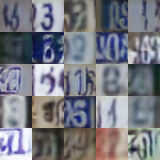
\includegraphics[width=0.2\textwidth]{imgs/s3_after-590-batches.png}}
  \mycaption{Comparison of SVHN data and generated samples from DCGAN}{}
  \label{fig_DCGAN_SVHN}
\end{figure}

The quality of the generated samples are not as good as the MNIST samples since the SVHN dataset is more complicated.
This complexity makes the model harder to converge i.e. uses more epoches to get good generated samples.

Although complicated as the dataset is, the generated samples demonstrate some qualities such as the variety of the samples. There are different combinations of gree, white, and red background with white, blue, and red fonts.
There are also a proportion of one-digit images and a proportion of the two-digits images.

\section{WGAN}

Wasserstein GAN(WGAN) is a modified GAN introduced by Arjovsky, Martin, et al.(2017)[5]. It proposed Wasserstein distance that has a better property, theoretically, than Jensen-Shannon divergence to measure the distance between two distributions. 

There is a common problem for naive version of GANs called collapse mode, and at the beginning of training, its quite hard for generator to learn something. Roughly speaking, this is all caused by gradient saturation which is brought by the property of Jensen-Shannon divergence that for two distributions with no overlap, the JS divergence is always infinity. 

In order to use Wasserstein distance, 1-Lipschitz function are required and for the purpose of implementation, gradient penalty is utilized and all we need to do is to modify the loss function a little bit. All the structures and the hyper-parameters are exactly the same as DCGAN.  

\begin{figure}[!htb]
  \centering
  \subfloat[MNIST data]{
  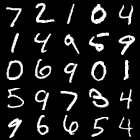
\includegraphics[width=0.2\textwidth]{imgs/mnist_data.png}}
  \subfloat[Epoch 10/50]{
  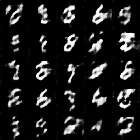
\includegraphics[width=0.2\textwidth]{imgs/I5_after-31-batches.png}}
  \subfloat[Epoch 30/50]{
  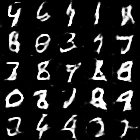
\includegraphics[width=0.2\textwidth]{imgs/I6_after-101-batches.png}}
  \subfloat[Epoch 50/50]{
  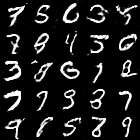
\includegraphics[width=0.2\textwidth]{imgs/I7_after-149-batches.png}}
  \mycaption{Comparison of MNIST data and generated samples from WGAN}{}
  \label{fig_MNIST}
\end{figure}

\subsection{WGAN on MNIST}
As of the samples shown in Figure \ref{fig_MNIST}, there is no significant difference between the two models. Both qualities are satisfying. The MNIST is so simple that even the most naive GANs can get a good performance with some tuning of parameters. So, at least for us, DCGAN would be our first choice. 

The Figure \ref{fig_GANs_MNIST} shows that the comparison of DCGAN and WGAN on MNIST. Both are trained for 50 epochs. For the implementation purpose, the original WGAN use weight clipping and a better version is to add gradient penalty. In order to calculate that penalty, a sampling process is required and thus in generally speaking, WGAN will sacrifice some efficiency. 

\begin{figure}[!htb]
  \centering
  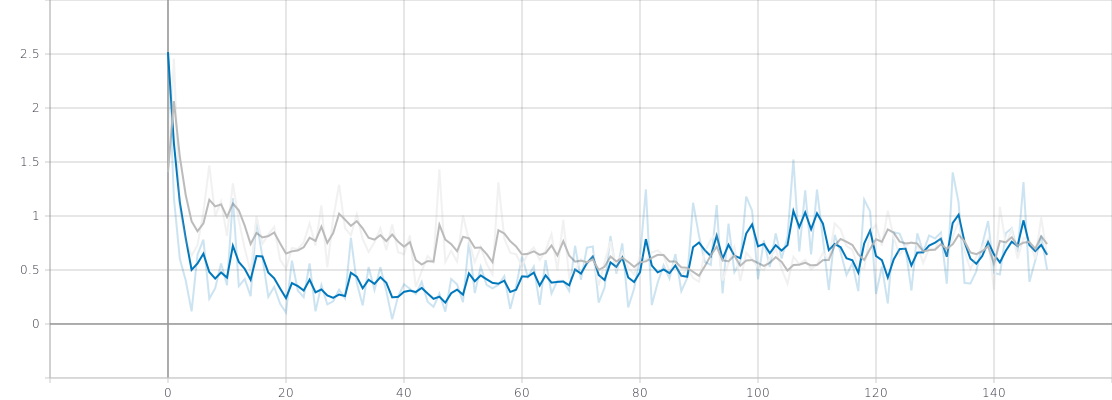
\includegraphics[width=0.8\textwidth]{imgs/mnist-train-discriminator-loss.png}
  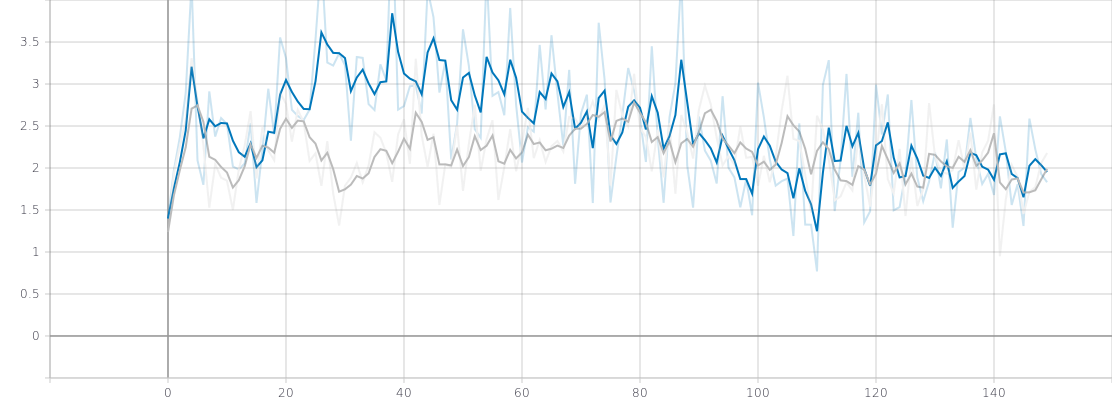
\includegraphics[width=0.8\textwidth]{imgs/mnist-train-generator-loss.png}
  \mycaption{Comparison of WGAN and DCGAN on MNIST with 50 epochs}{The two graphs are downloaded from tesorboard and the above one shows the loss of discriminator and the bellow on shows the loss of generator. The gray line is the for DCGAN and the blue line is for WGAN.}  
  \label{fig_GANs_MNIST}
\end{figure}

\subsection{WGAN on SVHN}

\begin{figure}[!htb]
  \centering
  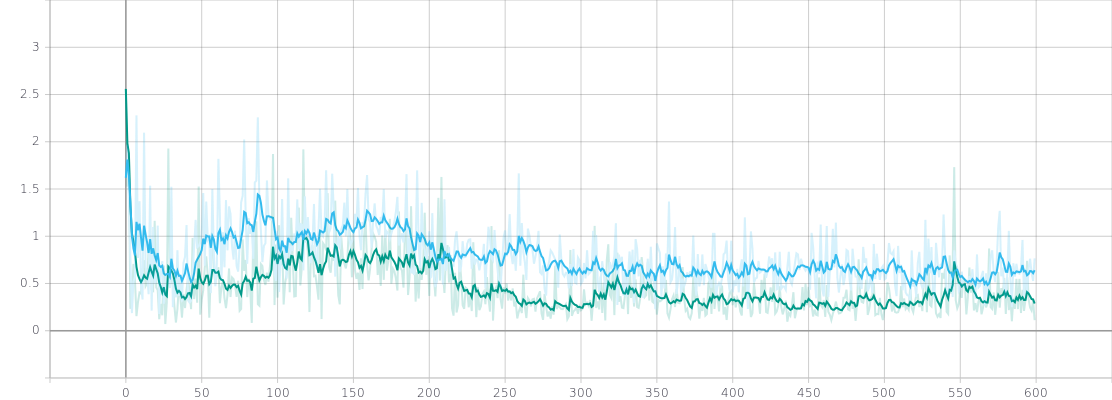
\includegraphics[width=0.8\textwidth]{imgs/svhn-train-discriminator-loss.png}
  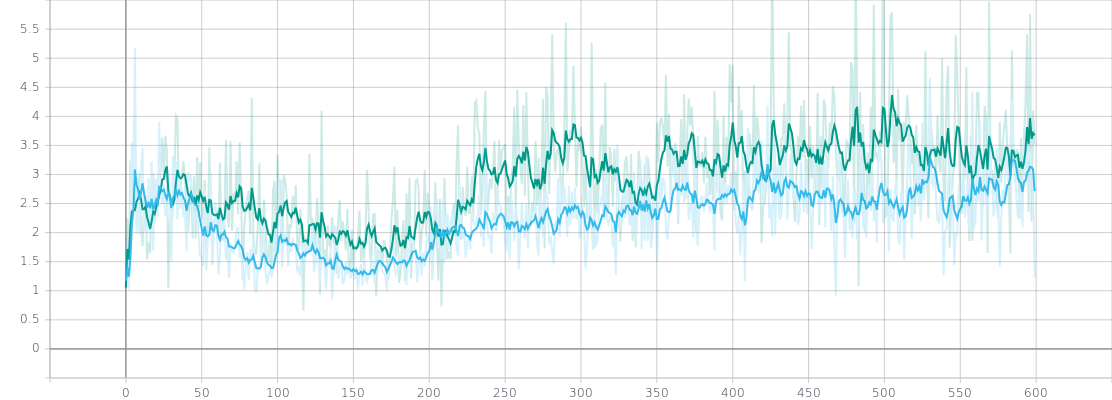
\includegraphics[width=0.8\textwidth]{imgs/svhn-train-generator-loss.png}
  \mycaption{Comparison of WGAN and DCGAN on SVHN with 200 epochs}{The two graphs are downloaded from tesorboard and the above one shows the loss of discriminator and the bellow on shows the loss of generator. The blue line is the for DCGAN and the green line is for WGAN.}  
  \label{fig_GANs_SVHN}
\end{figure}

\begin{figure}[!htb]
  \centering
  \subfloat[SVHN data]{
  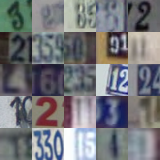
\includegraphics[width=0.2\textwidth]{imgs/svhn_data.png}}
  \subfloat[Epoch 30/200]{
  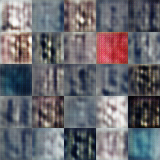
\includegraphics[width=0.2\textwidth]{imgs/s4_after-103-batches.png}}
  \subfloat[Epoch 150/200]{
  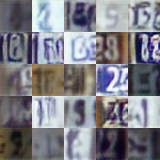
\includegraphics[width=0.2\textwidth]{imgs/s5_after-514-batches.png}}
  \subfloat[Epoch 200/200]{
  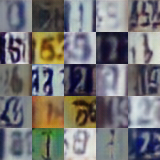
\includegraphics[width=0.2\textwidth]{imgs/s6_after-590-batches.png}}
  \mycaption{Comparison of SVHN data and generated samples from WGAN}{}
\end{figure}

The observation is similar for on the SVHN, even the dataset is more challenging, the DCGAN can converge fast and steady during the training process, the variability of the reconstructed samples are wide/large. Thus, there is no need to use a more complicate and sophisticate structure GAN. 

\section{Summary}

In short, we have studied the generative adversarial nets, especially the DCGAN and WGAN. We implemented these two models to the MNIST and SVHN dataset respectively and obtained satisfying samples.

Throughout the project, we have only tuned a few hyperparameters such as learning rate and batches. In the next step, we would tune the dimension of the noise, the structure of the model, etc.

Since plenty new models have been published other than WGAN, in the future, we can try other models such as triple-GAN[6], self-attention neural networkn[7], LOGAN[8] etc.

\section*{References}

[1] Goodfellow, Ian, et al. "Generative adversarial nets." Advances in neural information processing systems. 2014.

[2] LeCun, Yann, et al. “THE MNIST DATABASE.” MNIST Handwritten Digit Database, http://yann.lecun.com/exdb/mnist/.

[3] Netzer, Yuval, et al. "Reading digits in natural images with unsupervised feature learning." (2011).

[4] Radford, Alec, Luke Metz, and Soumith Chintala. "Unsupervised representation learning with deep convolutional generative adversarial networks." arXiv preprint arXiv:1511.06434 (2015).

[5] Arjovsky, Martin, Soumith Chintala, and Léon Bottou. "Wasserstein gan." arXiv preprint arXiv:1701.07875 (2017).

[6] Chongxuan, L. I., et al. "Triple generative adversarial nets." Advances in neural information processing systems. 2017.

[7] Zhang, Han, et al. "Self-attention generative adversarial networks." arXiv preprint arXiv:1805.08318 (2018).

[8] Wu, Yan, et al. "LOGAN: Latent Optimisation for Generative Adversarial Networks." arXiv preprint arXiv:1912.00953 (2019).

\end{document}